\parbox{\textwidth}{\footnotesize\sffamily 
  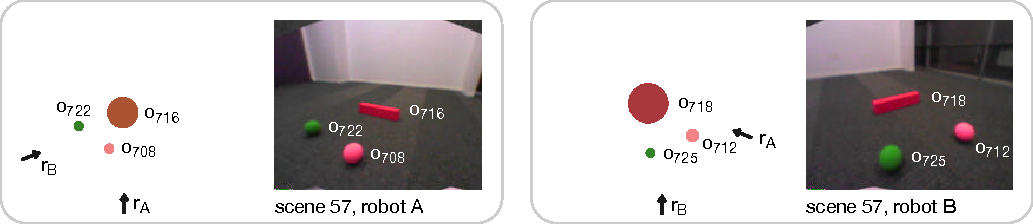
\includegraphics[width=1\textwidth]{figures/vision-system-example-scene}
  \vspace{1mm}
  
  \renewcommand{\arraystretch}{1.5}
  \newcommand{\sub}[1]{\raisebox{-2pt}{\scriptsize{#1}}}
  \addtolength{\tabcolsep}{-1.3pt}
  \definecolor{dark}{rgb}{0.5,0.2,0}     
  \begin{tabular*}{\textwidth}{@{}p{26.5mm}|rl|rl|rl||rll|rll|rll@{}}
    & \multicolumn{6}{c||}{experience robot A} & \multicolumn{9}{c}{experience robot B} \\
    feature \normalsize & 
    \multicolumn{2}{c}{o\sub{708}} & 
    \multicolumn{2}{c}{o\sub{716}} &
    \multicolumn{2}{c||}{o\sub{722}} & 
    \multicolumn{3}{c}{o\sub{712}} & 
    \multicolumn{3}{c}{o\sub{718}} & 
    \multicolumn{3}{c}{o\sub{725}} \\
    \hline
    x & 464 & 0.43 & 821 & 0.69 & 686 & 0.59
    & 607 & 0.53 & \itshape\textcolor{dark}{0.11}
    & 925 & 0.76 & \itshape\textcolor{dark}{0.08}
    & 432 & 0.40 & \itshape\textcolor{dark}{0.19} \\
    y & 151 & 0.61 & 17 & 0.51 & 453 & 0.82
    & -301 & 0.28 & \itshape\textcolor{dark}{0.33}
    & 137 & 0.60 & \itshape\textcolor{dark}{0.09}
    & 115 & 0.58 & \itshape\textcolor{dark}{0.25} \\
    width & 47 & 0.31 & 150 & 1.00 & 46 & 0.30
    & 62 & 0.46 & \itshape\textcolor{dark}{0.15}
    & 196 & 1.00 & \itshape\textcolor{dark}{0.00}
    & 45 & 0.29 & \itshape\textcolor{dark}{0.01} \\
    height & 116 & 0.35 & 138 & 0.42 & 67 & 0.19
    & 109 & 0.33 & \itshape\textcolor{dark}{0.02}
    & 186 & 0.58 & \itshape\textcolor{dark}{0.16}
    & 135 & 0.41 & \itshape\textcolor{dark}{0.22} \\
    luminance & 126 & 0.76 & 72 & 0.30 & 81 & 0.37
    & 130 & 0.79 & \itshape\textcolor{dark}{0.03}
    & 57 & 0.17 & \itshape\textcolor{dark}{0.13}
    & 85 & 0.41 & \itshape\textcolor{dark}{0.03} \\
%     stdev-luminance & 41 & 0.71 & 23 & 0.39 & 22 & 0.36
%     & 39 & 0.69 & \itshape\textcolor{dark}{0.03}
%     & 15 & 0.24 & \itshape\textcolor{dark}{0.15}
%     & 20 & 0.33 & \itshape\textcolor{dark}{0.04} \\
%     min-luminance & 35 & 0.40 & 40 & 0.48 & 29 & 0.31
%     & 26 & 0.26 & \itshape\textcolor{dark}{0.14}
%     & 39 & 0.46 & \itshape\textcolor{dark}{0.02}
%     & 27 & 0.27 & \itshape\textcolor{dark}{0.03} \\
%     max-luminance & 199 & 0.79 & 185 & 0.69 & 126 & 0.30
%     & 198 & 0.78 & \itshape\textcolor{dark}{0.01}
%     & 139 & 0.39 & \itshape\textcolor{dark}{0.30}
%     & 126 & 0.30 & \itshape\textcolor{dark}{0.00} \\
    green-red & 206 & 0.81 & 187 & 0.72 & 101 & 0.29
    & 206 & 0.81 & \itshape\textcolor{dark}{0.00}
    & 196 & 0.76 & \itshape\textcolor{dark}{0.04}
    & 98 & 0.28 & \itshape\textcolor{dark}{0.01} \\
%     stdev-green-red & 17 & 0.71 & 22 & 0.93 & 8 & 0.29
%     & 17 & 0.71 & \itshape\textcolor{dark}{0.00}
%     & 9 & 0.35 & \itshape\textcolor{dark}{0.58}
%     & 8 & 0.30 & \itshape\textcolor{dark}{0.01} \\
%     min-green-red & 149 & 0.76 & 129 & 0.64 & 80 & 0.34
%     & 139 & 0.70 & \itshape\textcolor{dark}{0.06}
%     & 151 & 0.77 & \itshape\textcolor{dark}{0.13}
%     & 76 & 0.31 & \itshape\textcolor{dark}{0.02} \\
%     max-green-red & 233 & 0.79 & 253 & 0.89 & 126 & 0.27
%     & 232 & 0.79 & \itshape\textcolor{dark}{0.00}
%     & 252 & 0.89 & \itshape\textcolor{dark}{0.00}
%     & 123 & 0.26 & \itshape\textcolor{dark}{0.01} \\
    yellow-blue & 119 & 0.53 & 110 & 0.47 & 99 & 0.38
    & 121 & 0.55 & \itshape\textcolor{dark}{0.02}
    & 123 & 0.57 & \itshape\textcolor{dark}{0.10}
    & 97 & 0.37 & \itshape\textcolor{dark}{0.02} \\
%     stdev-yellow-blue & 4 & 0.32 & 22 & 1.00 & 9 & 0.53
%     & 4 & 0.31 & \itshape\textcolor{dark}{0.00}
%     & 4 & 0.29 & \itshape\textcolor{dark}{0.71}
%     & 9 & 0.53 & \itshape\textcolor{dark}{0.00} \\
%     min-yellow-blue & 100 & 0.56 & 39 & 0.12 & 72 & 0.36
%     & 102 & 0.58 & \itshape\textcolor{dark}{0.01}
%     & 95 & 0.53 & \itshape\textcolor{dark}{0.41}
%     & 72 & 0.36 & \itshape\textcolor{dark}{0.00} \\
%     max-yellow-blue & 132 & 0.45 & 133 & 0.46 & 124 & 0.38
%     & 132 & 0.45 & \itshape\textcolor{dark}{0.00}
%     & 140 & 0.52 & \itshape\textcolor{dark}{0.06}
%     & 126 & 0.40 & \itshape\textcolor{dark}{0.02} \\
    \hline
  \end{tabular*}
  \vspace{3mm}
  
}


% (defparameter *world* (make-instance 'physical-robot-world :data-sets '("qrio-1")))
%
% (defparameter *objects* (list (third (entities (get-world-model *world* "scene-3378523360" 'a)))
% 			    (fifth (entities (get-world-model *world* "scene-3378523360" 'a)))
% 			    (fourth (entities (get-world-model *world* "scene-3378523360" 'a)))
% 			    (third (entities (get-world-model *world* "scene-3378523360" 'b)))
% 			    (fifth (entities (get-world-model *world* "scene-3378523360" 'b)))
% 			    (fourth (entities (get-world-model *world* "scene-3378523360" 'b)))))
%
% (loop for i from 0 to 16
%    do (format t "~%      ~(~a~)" (fname (nth i (features (first *objects*)))))
%      (loop for object in (subseq *objects*  0 3)
% 	do (format t " & ~d & ~,2f" (round (value (fvalue (nth i (features object))))) (value (fvalue (nth (+ i 17) (features object))))))
%      (loop for object in (subseq *objects*  3 6)
% 	for j from 3
% 	do (format t "~%      & ~d & ~,2f & \\itshape\\textcolor{dark}{~,2f}" (round (value (fvalue (nth i (features object))))) 
% 		   (value (fvalue (nth (+ i 17) (features object))))
% 		   (abs (- (value (fvalue (nth (+ i 17) (features object)))) (value (fvalue (nth (+ i 17) (features (nth (- j 3) *objects*)))))))))
%      (format t " \\\\"))

%%% Local Variables: 
%%% mode: latex
%%% TeX-master: "../phd-thesis"
%%% End: 
